\mode*
\begin{frame}[label=MR1]
  \MRoneTime
  \frametitle{Viabilidad}
  \framesubtitle{Coherencia de desarrollos previos}
  \quad\hspace{-0.8cm}\vspace{-0.5cm}
  \begin{columns}[T,totalwidth=0.97\textwidth]
    \small
    \begin{column}{0.55\textwidth}\setbeamercovered{transparent}
      \begin{itemize}
      \item<1-|alert@1|uncover@1-6> Desarrollos de plataformas rob\'oticas seriales y paralelas
        \only<2-6>{
          \textit{\textbf{Ejemplo proceso de dise\~no:}}\setbeamercovered{transparent}
          \begin{enumerate}\scriptsize
          \item<2-|alert@2|uncover@2-3> Bajo costo
          \item<3-|alert@3|uncover@3> Didacticos
          \item<4-|alert@4|uncover@4> Modularidad
          \item<5-|alert@5|uncover@5> Prototipado rapido
          \item<6-|alert@6|uncover@6> Metodologia de dise\~no
          \end{enumerate}
        }
      \end{itemize}
    \end{column}
    \begin{column}{0.4\textwidth}
      \parbox[c][7cm][c]{4.0cm}{
        \only<1-4>{
          \begin{center}
            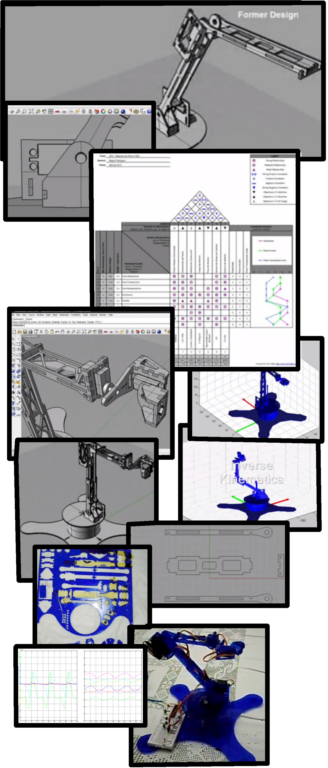
\includegraphics[height=7cm]{../images/RobotMR1_0.png}
          \end{center}
        }
        \only<5>{
          % 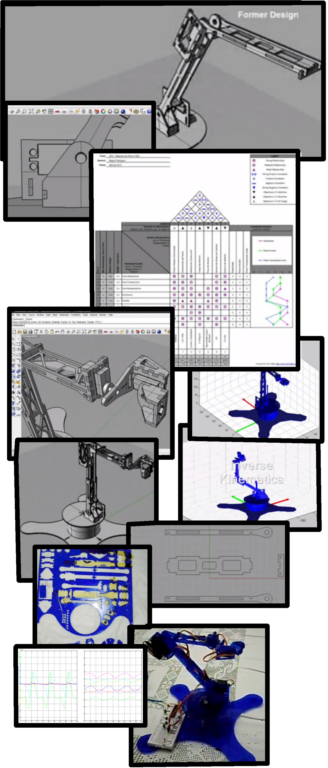
\includegraphics[height=7cm]{../images/RobotMR1_0.png}
          \begin{center}
            \animategraphics[height=7cm,autoresume,autoplay]{3}{../images/RobotMR1_}{0}{12}
          \end{center}
        }
        \only<6>{
          \begin{center}
            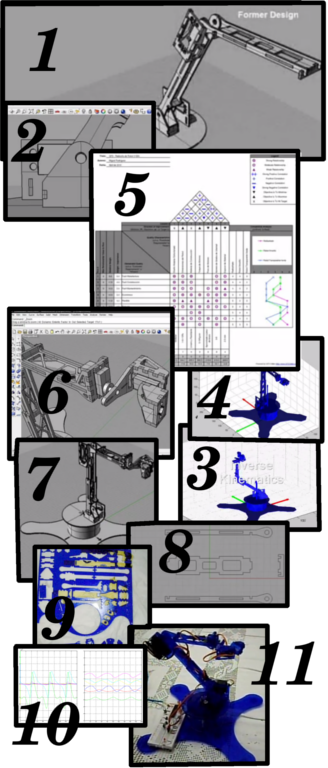
\includegraphics[height=7cm]{../images/RobotMR1_12.png}
          \end{center}
          % \movie[width=3cm,height=7cm,externalviewer]{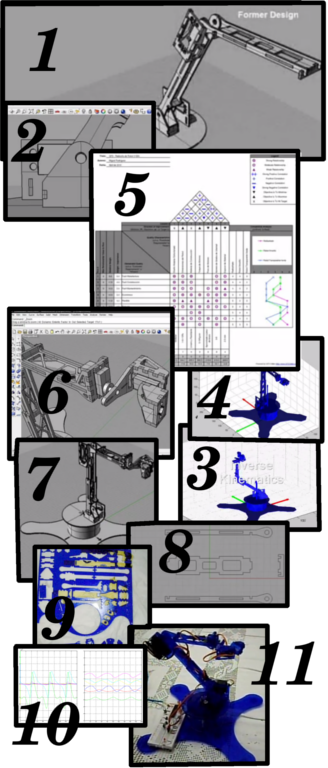
\includegraphics[height=7cm]{../images/RobotMR1_12.png}}{../videos/RobotMR1.flv} 
        }
      }
    \end{column}
  \end{columns}
\end{frame}
